\documentclass[notes]{beamer}

\usepackage{default}
\usepackage{pgfpages}
\usepackage{pgf-pie}
\usepackage{ifthen}

\usetheme{Szeged}
\usecolortheme{dolphin}
\setbeamertemplate{note page}{\pagecolor{yellow!25}\insertnote}
%\setbeamertemplate{note page}{\pagecolor{white}\insertnote}

\title{Natural Language processing for Knowledge Representation}
\subtitle{Tussentijdse presentatie}

\author{Jens Claes}
\date{19 december 2016}

\newcommand{\seperation}{
	\vspace{1em}
	\ppause
}
\newcommand{\sseperation}{
	\vspace{1em}
}
\newcommand{\hitem}{
	\ppause
	\item
}
\newcommand{\ppause}{\onslide<+>}
\newcommand{\nnote}[1]{\note<.>{#1}}
\setbeamercovered{%
	still covered={\opaqueness<1->{0}},
	again covered={\opaqueness<1->{60}}
}
\setbeameroption{hide notes} % Only slides
\setbeameroption{show notes on second screen=right} % Both

%\graphicspath{ {../images/} }

\setbeamertemplate{bibliography item}{\insertbiblabel}
\begin{document}
	\frame{\titlepage}
	\section{Probleem}
	\begin{frame}{Situatie I}
		\begin{itemize}
			\hitem Specificaties in natuurlijke taal
			\item Door domein expert
			
			\seperation
			
			\item Vertaald naar programma's
			\item Inconsistent, moeilijk aanpasbaar
			
			\seperation
			
			\item Antwoord: Knowledge base paradigma
		\end{itemize}
		
		\note<1>{Businesses = ruled by requirements / specifications}
		\note<2>{Vroeger: omzetten naar verschillende programma's: incosistenties + moeilijk aanpasbaar, ...}
		\note<3>{KBS paradigma lost deze problemen op... maar creëert er nieuwe}
	\end{frame}
	\begin{frame}{Situatie II: KBS paradigma}
			\begin{itemize}
				\hitem Requirements in natuurlijke taal
				\item Door domein expert
				\nnote{KBS: nog steeds in natuurlijke taal. Niet meer per se alles al vastgelegd als een specificatie}
				
				\seperation
				
				\item Vertaald naar formele taal
				\item Door KBS expert
				\nnote{Iemand anders doet vertaling. Tweede specificatie + extra werk}
				
				\seperation
				
				\item Domein expert: geen formele taal
				\item KBS expert: geen domeinkennis
				\item $\Rightarrow$ Feedback loop beperkt
				\nnote{KBS kent domein niet en domain expert kent logica niet: moeilijk om feedback te geven over tweede vertaling}
				
				\seperation
				
				\item Kunnen we een formele taal ontwerpen die toegankelijk is voor domein experts, rijk genoeg is voor praktische problemen en toepasbaar is binnen KBS
				\nnote{Probleemstelling thesis}
				
				\seperation
				
				\item Antwoord: Formele \textbf{natuurlijke} talen?
				\nnote{Een formele taal nodig die toegankelijk is voor domain expert. Op zijn minst om feedback te kunnen geven over de vertaling, op zijn best om de KBS expert uit het plaatje te verwijderen}
			\end{itemize}
	\end{frame}
	
	\begin{frame}{Waarom}
		\begin{itemize}
			\hitem Natuurlijke taal al gebruikt. 
			\item Stel (ook) formele specificatie erin op.
			\begin{figure}
				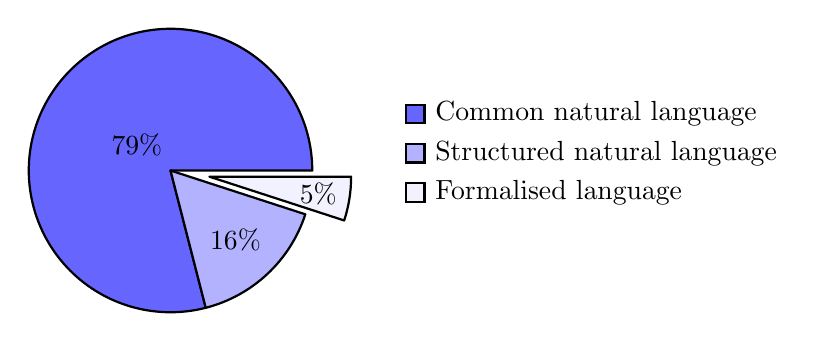
\begin{tikzpicture}
				    \pie[text = legend, radius = 1.8, explode = {0, 0, 0.5}, color = {blue!60, blue!30, blue!5}]{79/Common natural language, 16/Structured natural language, 5/Formalised language}
				\end{tikzpicture}
				\caption{Use of language in Requirements Engineering in 1999 (From figure 5 in \cite{Luisa2004})}
			\end{figure}
			
			\hitem Leesbaar voor domein expert, KBS expert en machines
		\end{itemize}
		
		\note<1>{
			\begin{itemize}
				\item Domein experts stellen de specificatie op. Zij kennen geen formele talen.
				\item Controlled natural language is wel mogelijk. Soms wordt het al gebruikt. Meestal minder formele talen dan. Enkel voor de leesbaarheid.
			\end{itemize}
		}
		\note<2>{Machines kunnen specificaties lezen en omzetten als input voor KBS}
	\end{frame}
	
	\section{Doel}
	\begin{frame}{Doel Thesis}
		\begin{itemize}
			\hitem Nieuwe taal construeren
			\item Basis FO concepten
			\item Toegankelijk voor domein experten
			
			\seperation
			\item Kunnen we $FO(.)^{IDP3}$ \cite{Bruynooghe2014} constructs toevoegen?
			\item Kunnen we een NLP interface aanbieden voor IDP?
			
			\seperation
			\item Kunnen we dynamische systemen toevoegen?
		\end{itemize}
		\note<1>{Nieuwe formele natuurlijke taal met een simpele BNF zodat lookahead mogelijk is, indien later nog gewenst: Makkelijker te leren + tools rond te bouwen}
		\note<2>{
			\begin{itemize}
				\item Arithmetic toevoegen? (al deels in ACE)
				\item Aggregates toevoegen?
				\item Types toevoegen?
				\item Partial functions toevoegen?
				\item Inductive definitions toevoegen?
				\item NLP vragen als entrypoint voor verschillende inferenties?
				\item Kunnen we vocabulary en structures voorstellen? Of er automatisch uithalen?
			\end{itemize}
			$\Rightarrow$ Hoe volledig kunnen we de interface naar IDP maken?
		}
		\note<3>{Extra: Kunnen we dynamische systemen modelleren met natuurlijke taal (gebruik makend van Event-based ipv LTC).}
	\end{frame}

  \section{Voorbeeld}

  \begin{frame}{Zebra puzzel\cite{ZebraPuzzle}}
    \ppause
    \nnote{Zebra puzzel of einstein puzzle is een bekende puzzle. Om het werk dat al gebeurd is het voorbije semester te illustreren altijd aan de hand van voorbeelden.
    \\ _
    \\ De tool werkt zeker nog niet perfect maar kan het grootste deel van de zebra puzzle al vertalen. In het kort vertaald het werkwoorden en adjectieven naar predicaten en zelfstandige naamwoorden naar een waarde uit constructed type of variabelen. De structuur van de formule wordt bepaald door de structuur van de quantoren en de vuistregels van logica
    \\ _
    \\ De eerste lijn is zin volgens wikipedia, tweede zoals ingegeven in de tool, derde is de vertaling in logica die de tool genereert. \\
    }
    \begin{enumerate}
      \hitem There are five houses.
      \nnote{Moeilijk af te dwingen met de theorie. Dit is iets voor vocabularium of structuur}

      \hitem The Spaniard owns the dog. \\ The Spaniard keeps the dog. \\ $keeps(spaniard,dog).$ \\
      \item The Japanese smokes Parliaments. \\ The Japanese smokes Parliaments. \\ $smokes(japanese,parliaments).$ \\
      \item The Ukrainian drinks tea. \\ The Ukrainian drinks tea. \\ $drinks(ukrainian,tea).$ \\
      \nnote{Werkwoorden mappen op predicaten}
    \end{enumerate}
  \end{frame}
  \begin{frame}{Zebra puzzel\cite{ZebraPuzzle}}
    \begin{enumerate}
      \setcounter{enumi}{4}
      \hitem The Englishman lives in the red house. \\ The Englishman lives in the red house. \\ $\forall x1: color(x1,red) \Rightarrow lives(englishman,x1).$ \\
      \item The Norwegian lives in the first house. \\ The Norwegian lives in the first house. \\ $\forall x1: position(x1,first) \Rightarrow lives(norwegian,x1).$ \\
      \item The Lucky Strike smoker drinks orange juice. \\ The person who smokes Lucky Strike, drinks Orange Juice. \\ $\forall x1: smokes(x1,[lucky,strike]) \Rightarrow drinks(x1,[orange,juice]).$ \\
      \nnote{Adjectieven mappen ook op predicaten. Voorlopig op binaire predicaten, unaire predicaten kan logischer zijn, maar dan moet er nog connectie gemaakt worden met de binaire predicaten
      \\ Bepaalde lidwoorden wordt voorlopig op forall gemapt, moet nog verder onderzocht worden in minder artificieel probleem}
    \end{enumerate}
  \end{frame}
  \begin{frame}{Zebra puzzel\cite{ZebraPuzzle}}
    \begin{enumerate}
      \setcounter{enumi}{7}
      \hitem The Old Gold smoker owns snails. \\ There is a person who smokes Old Gold and keeps the snail. \\ $\exists x1: keeps(x1,snail) \land smokes(x1,[old,gold]).$ \\
      \nnote{Onbepaalde lidwoorden mapt op existentiele. And wordt vertaald naar logische and}
      \hitem Coffee is drunk in the green house. \\ There is a person who lives in the green house and drinks coffee. \\ $\exists x1: drinks(x1,coffee) \land [\forall x2: color(x2,green) \Rightarrow lives(x1,x2)].$ \\
      \item Kools are smoked in the yellow house. \\ There is a person who lives in a yellow house and smokes Kools. \\ $\exists x1: smokes(x1,kools) \land [\exists x2: color(x2,yellow) \land lives(x1,x2)].$ \\
      \nnote{2 zinnen met dezelfde structuur. 2e deel komt naar voor door manier van opbouwen van formules}
    \end{enumerate}
  \end{frame}
  \begin{frame}{Zebra puzzel\cite{ZebraPuzzle}}
    \begin{enumerate}
      \setcounter{enumi}{8}
      \hitem Milk is drunk in the middle house. \\ The person who lives in the third house, drinks milk. \\ $\forall x1: drinks(x1,milk) \Rightarrow [\forall x2: position(x2,third) \Rightarrow lives(x1,x2)].$ \\
      \nnote{Nog een foute vertaling. In deze context klopt het wel maar niet de vertaling van de EN zin. Kan opgelost worden voor deze zin door ``the'' op exists te mappen maar zou nog altijd problemen geven bij Every person who...}
      \hitem The Norwegian lives next to the blue house. \\ The Norwegian lives in a house that is next to the blue house. \\ $\exists x1: lives(norwegian,x1) \land [\forall x2: color(x2,blue) \Rightarrow [is,next,to](x1,x2)].$ \\
    \end{enumerate}
  \end{frame}
  \begin{frame}{Zebra puzzel\cite{ZebraPuzzle}}
    \begin{enumerate}
      \setcounter{enumi}{12}
      \hitem The green house is immediately to the right of the ivory house. \\ The position of the green house is equal to the position of the ivory house plus 1. \\ $\forall x1: color(x1,green) => [\forall x2: color(x2,ivory) => position(x1)=position(x2)+1].$
      \nnote{er zit al een beetje aritmetiek in de taal. Kan nog uitgebreid worden}
    \end{enumerate}
  \end{frame}
  \begin{frame}{Zebra puzzel\cite{ZebraPuzzle}}
    \begin{enumerate}
      \setcounter{enumi}{13}
      \hitem \textit{Wereldkennis} \\ A house A is next to a house B if the absolute value of the difference between the position of house A and the position of house B is equal to 1. \\ $\forall a, b: [is,next,to](a, b) \leftarrow |position(a)-position(b)|=1.$
      \nnote{``Next to'' is concept uit de wereld die we expliciet moeten vertalen. Vertaling naar logica werkt nog niet}
      \hitem The man who smokes Chesterfields lives in the house next to the man with the fox. \\ The house in which the person who smokes Chesterfields lives, is next to the house in which the person who keeps the fox lives. \\ $\forall x1: \forall x2: smokes(x2,chesterfields) \Rightarrow [lives(x2,x1) \land \forall x3: [is,next,to](x1,x3) \land \{\forall x4: keeps(x4,fox) \Rightarrow lives(x4,x3)\}].$
      \nnote{veruit de moeilijkste zin uit Zebra Puzzle}
    \end{enumerate}
  \end{frame}
  \begin{frame}{Zebra puzzel\cite{ZebraPuzzle}}
    \begin{enumerate}
      \setcounter{enumi}{15}
      \hitem Kools are smoked in the house next to the house where the horse is kept. \\ The house in which the person who smokes Kools lives, is next to the house in which the person who keeps a horse lives. \\ $ \forall x1: \forall x2: smokes(x2,kools) \Rightarr\Rightarr\Rightarr\Rightarr\Rightarr\Rightarr\Rightarr\Rightarr\Rightarrow [lives(x2,x1) \land \forall x3: [is,next,to](x1,x3) \land \{\forall x4: keeps(x4,horse) \Rightarrow lives(x4,x3)\}].$ \\
      \nnote{zelfde structuur als vorige zin}
      
      \hitem \textit{Domeinkennis} \\ Every animal is kept by exactly 1 person. \\ $\forall x1: \exists=1 x2: kept(x2,x1).$
      \nnote{kept: passief, kennis van vervoegingen nodig}
    \end{enumerate}
  \end{frame}

  \section{Planning}
  \begin{frame}{Planning}
			\begin{itemize}
        \hitem Blok- en examenperiode: niets
        \hitem Februari
          \begin{itemize}
            \item Vocabularium formaliseren
            \item Vocabularium gebruiken bij parsen theorie
            \item Natuurlijke taal interface voor vocabularium
          \end{itemize}
        \hitem Maart
          \begin{itemize}
            \item Expressiviteit formele taal verhogen
            \item Bv. Definities, aritmetiek, aggregaten, ...
          \end{itemize}
        \hitem April
          \begin{itemize}
            \item Schrijven thesis
            \item Taal uittesten op grote probleem (expressiviteit, leesbaarheid, ...)
          \end{itemize}
        \hitem Mei
          \begin{itemize}
            \item Schrijven thesis
          \end{itemize}
			\end{itemize}
  \end{frame}
			
	\section{Referenties}
	\begin{frame}[allowframebreaks]{Referenties}
		\bibliographystyle{plain}
		\bibliography{presentatie}
	\end{frame}
	
\end{document}
